\documentclass[12pt,letterpaper]{article}
\usepackage{graphicx,textcomp}
\usepackage{natbib}
\usepackage{setspace}
\usepackage{fullpage}
\usepackage{color}
\usepackage[reqno]{amsmath}
\usepackage{amsthm}
\usepackage{fancyvrb}
\usepackage{amssymb,enumerate}
\usepackage[all]{xy}
\usepackage{endnotes}
\usepackage{lscape}
\newtheorem{com}{Comment}
\usepackage{float}
\usepackage{hyperref}
\newtheorem{lem} {Lemma}
\newtheorem{prop}{Proposition}
\newtheorem{thm}{Theorem}
\newtheorem{defn}{Definition}
\newtheorem{cor}{Corollary}
\newtheorem{obs}{Observation}
\usepackage[compact]{titlesec}
\usepackage{dcolumn}
\usepackage{tikz}
\usetikzlibrary{arrows}
\usepackage{multirow}
\usepackage{xcolor}
\newcolumntype{.}{D{.}{.}{-1}}
\newcolumntype{d}[1]{D{.}{.}{#1}}
\definecolor{light-gray}{gray}{0.65}
\usepackage{url}
\usepackage{listings}
\usepackage{color}

\definecolor{codegreen}{rgb}{0,0.6,0}
\definecolor{codegray}{rgb}{0.5,0.5,0.5}
\definecolor{codepurple}{rgb}{0.58,0,0.82}
\definecolor{backcolour}{rgb}{0.95,0.95,0.92}

\lstdefinestyle{mystyle}{
	backgroundcolor=\color{backcolour},   
	commentstyle=\color{codegreen},
	keywordstyle=\color{magenta},
	numberstyle=\tiny\color{codegray},
	stringstyle=\color{codepurple},
	basicstyle=\footnotesize,
	breakatwhitespace=false,         
	breaklines=true,                 
	captionpos=b,                    
	keepspaces=true,                 
	numbers=left,                    
	numbersep=5pt,                  
	showspaces=false,                
	showstringspaces=false,
	showtabs=false,                  
	tabsize=2
}
\lstset{style=mystyle}
\newcommand{\Sref}[1]{Section~\ref{#1}}
\newtheorem{hyp}{Hypothesis}

\title{Problem Set 3}
\date{Due: November 19, 2022}
\author{Applied Stats/Quant Methods 1 \\ Dan Zhang 23335541}


\begin{document}
	\maketitle
	\section*{Instructions}
	\begin{itemize}
		\item Please show your work! You may lose points by simply writing in the answer. If the problem requires you to execute commands in \texttt{R}, please include the code you used to get your answers. Please also include the \texttt{.R} file that contains your code. If you are not sure if work needs to be shown for a particular problem, please ask.
	\item Your homework should be submitted electronically on GitHub.
	\item This problem set is due before 23:59 on Sunday November 19, 2023. No late assignments will be accepted.

	\end{itemize}

		\vspace{.25cm}
	
\noindent In this problem set, you will run several regressions and create an add variable plot (see the lecture slides) in \texttt{R} using the \texttt{incumbents\_subset.csv} dataset. Include all of your code.

	\vspace{.5cm}
\section*{Question 1}
\vspace{.25cm}
\noindent We are interested in knowing how the difference in campaign spending between incumbent and challenger affects the incumbent's vote share. 
	\begin{enumerate}
		\item Run a regression where the outcome variable is \texttt{voteshare} and the explanatory variable is \texttt{difflog}.	\vspace{.15cm}
		
	   \noindent  We can use the lm() function in R to see the regression between \texttt{voteshare} and \texttt{difflog}. Run the following codes in R then we can get the results of regression1.\\	\vspace{.15cm}
		
		\lstinputlisting[language=R,firstline=37,lastline=39,]{PS3.R}
		
		\noindent We can get the following results:\\ \vspace{.15cm}
		\begin{verbatim}
			Call:
			lm(formula = voteshare ~ difflog, data = inc.sub)
			
			Residuals:     
			   	Min      1Q      Median    3Q     Max 
			-0.26832 -0.05345 -0.00377  0.04780  0.32749 
			
			Coefficients:
			            Estimate Std. Error t value Pr(>|t|)    
		(Intercept) 0.579031   0.002251  257.19   <2e-16 ***
		difflog     0.041666   0.000968   43.04   <2e-16 ***
		---
		Signif. codes:  0 ‘***’ 0.001 ‘**’ 0.01 ‘*’ 0.05 ‘.’ 0.1 ‘ ’ 1
		
		Residual standard error: 0.07867 on 3191 degrees of freedom
		Multiple R-squared:  0.3673,	Adjusted R-squared:  0.3671 
		F-statistic:  1853 on 1 and 3191 DF,  p-value: < 2.2e-16
		\end{verbatim}
		\vspace{.5cm}
		
		\noindent From the results of regression1, we can see that the P-value (\textless 2.2e-16) is extremely low, providing strong evidence in favor of a significant relationship between \texttt{voteshare} and \texttt{difflog}\\ \vspace{.15cm}
		
		\item Make a scatterplot of the two variables and add the regression line. 	\vspace{.15cm}
		
		\noindent First, we draw the scatter plot of the two variables, and then using the abline() function to add the regression line. By running the following codes in R. We can get the graphic.\\
		
		\lstinputlisting[language=R,firstline=43,lastline=52]{PS3.R}
		
		\begin{figure}[h]
			\centering
			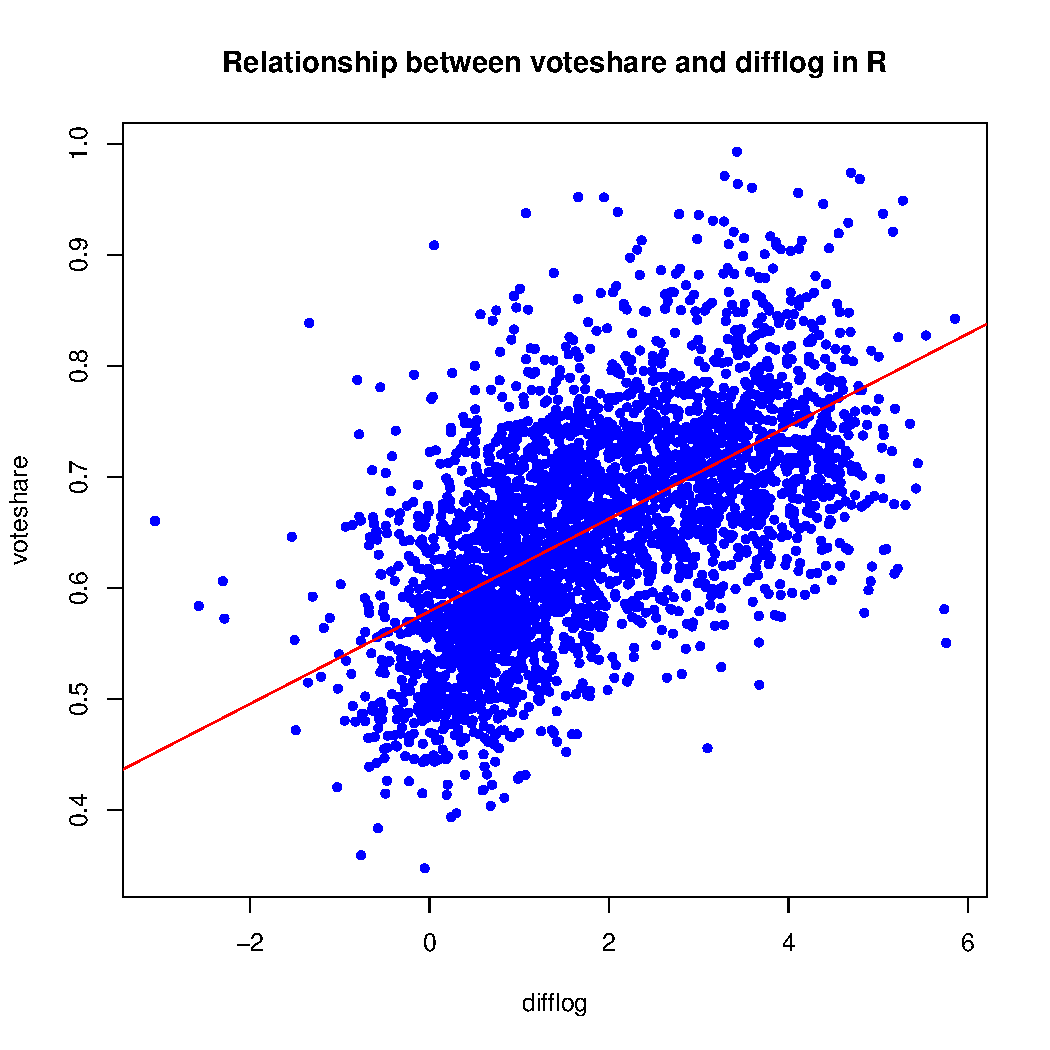
\includegraphics[width=0.8\textwidth]{Scatter plot and regression line of voteshare and difflog in R.pdf}
			\caption{Scatter plot and regression line of voteshare and difflog in R}
			\label{fig:pdf}
		\end{figure}
		
		\newpage
		\item Save the residuals of the model in a separate object.	\vspace{.17cm}
		
		\noindent Save the residuals of the regression1 in \texttt{residuals\textunderscore{}reg1} by running the following codes:\\
		
		\lstinputlisting[language=R,firstline=55,lastline=57]{PS3.R}
		
		\item Write the prediction equation.
		
		\noindent From the results of regression1 in Part 1.1, we can get the intercept and slope respectively. So the prediction equation would be:\\  
		\[ \hat{\texttt{voteshare}} = 0.579031 + 0.041666* \texttt{difflog} 
		\]\\ In this model, difflog has a positive effect on voteshare, with each unit difflog increase, increasing the voteshare estimate by 0.04167. The  voteshare estimate by 0.57903 when difflog is zero.\\
		
	\end{enumerate}

\section*{Question 2}
\noindent We are interested in knowing how the difference between incumbent and challenger's spending and the vote share of the presidential candidate of the incumbent's party are related.	\vspace{.25cm}
	\begin{enumerate}
		\item Run a regression where the outcome variable is \texttt{presvote} and the explanatory variable is \texttt{difflog}.	\vspace{.15cm}
		
		  \noindent  We can use the lm() function in R to see the regression between \texttt{presvote} and \texttt{difflog}. Run the following codes in R then we can get the results of regression2.	\vspace{.15cm}
		
		\lstinputlisting[language=R,firstline=64,lastline=66,]{PS3.R}
		
		\noindent We can get the following results: \vspace{.15cm}
		\begin{verbatim}
			Call:
			lm(formula = presvote ~ difflog, data = inc.sub)
			
			Residuals:
			     Min    1Q     Median    3Q    Max 
			-0.32196 -0.07407 -0.00102  0.07151  0.42743 
			
			Coefficients:
			            Estimate Std. Error t value Pr(>|t|)    
		(Intercept) 0.507583   0.003161  160.60   <2e-16 ***
		difflog     0.023837   0.001359   17.54   <2e-16 ***
		---
		Signif. codes:  0 ‘***’ 0.001 ‘**’ 0.01 ‘*’ 0.05 ‘.’ 0.1 ‘ ’ 1
		
		Residual standard error: 0.1104 on 3191 degrees of freedom
		Multiple R-squared:  0.08795,	Adjusted R-squared:  0.08767 
		F-statistic: 307.7 on 1 and 3191 DF,  p-value: < 2.2e-16
		\end{verbatim}
		\vspace{.15cm}
		
		\noindent From the results of regression2, we can see that the P-value (\textless 2.2e-16) is extremely low, providing strong evidence in favor of a significant relationship between \texttt{presvote} and \texttt{difflog}\\ \vspace{.15cm}
		
		\item Make a scatterplot of the two variables and add the regression line. 	\vspace{.15cm}
		
			\noindent First, we draw the scatter plot of the two variables, and then using the abline() function to add the regression line. By running the following codes in R. We can get the graphic.
		
		\lstinputlisting[language=R,firstline=69,lastline=78]{PS3.R}
		
		\begin{figure}[h]
			\centering
			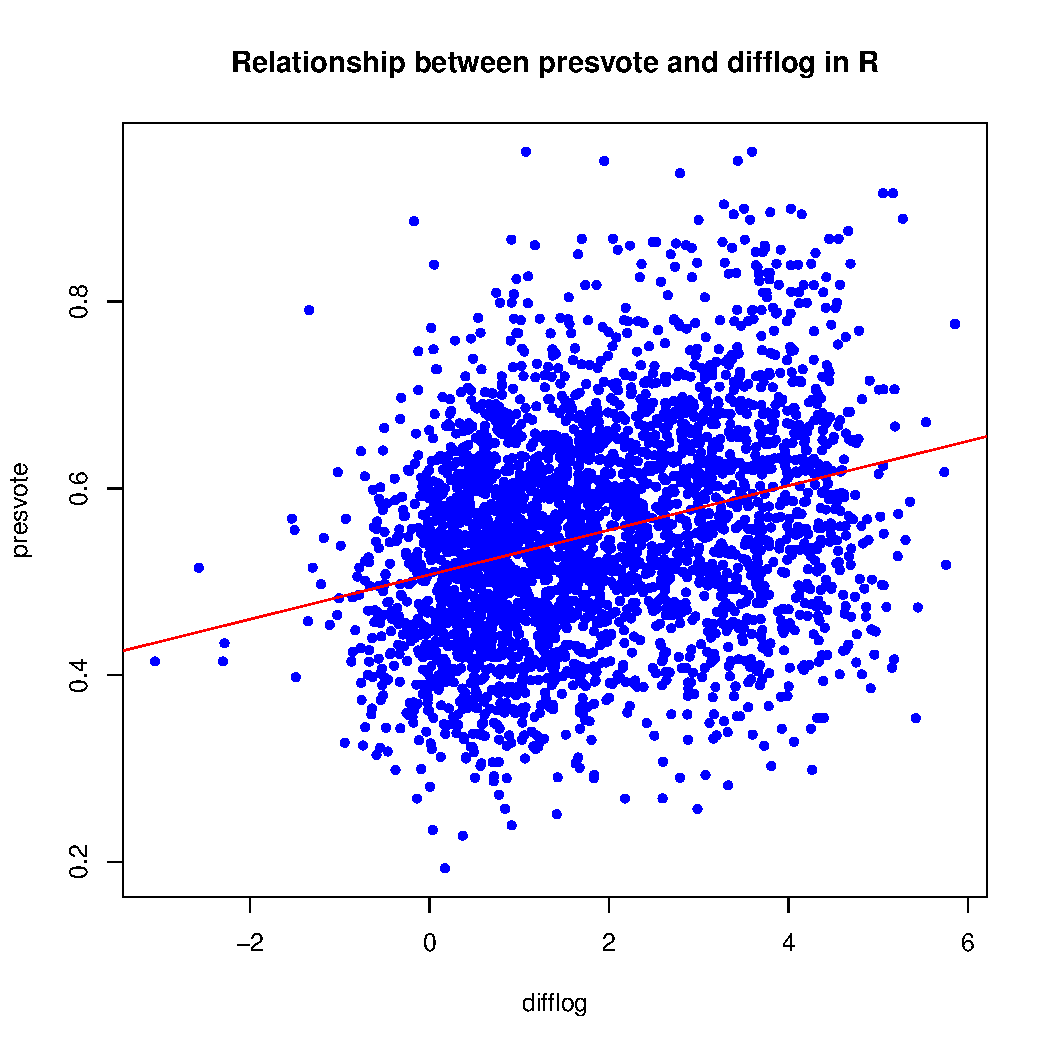
\includegraphics[width=0.8\textwidth]{Scatter plot and regression line of presvote and difflog in R.pdf}
			\caption{Scatter plot and regression line of presvote and difflog in R}
			\label{fig:pdf}
		\end{figure}
		
		\newpage
		\item Save the residuals of the model in a separate object.	\vspace{.15cm}
		
			\noindent Save the residuals of the regression2 in \texttt{residuals\textunderscore{}reg2} by running the following codes:
		
		\lstinputlisting[language=R,firstline=81,lastline=83]{PS3.R}
		
		\item Write the prediction equation.
		
		\noindent From the results of regression2 in Part 2.1, we can get the intercept and slope respectively. So the prediction equation would be:\\  \[\hat{\texttt{presvote}}= 0.507583 + 0.023837*\texttt{difflog}\]   \\In this model, difflog has a positive effect on presvote, the expected value of presvote would be 0.507583 when difflog is zero, with each addional unit change of difflog, the expected presvote changes by 0.023837.\\
		
	\end{enumerate}
	
	\newpage
\section*{Question 3}

\noindent We are interested in knowing how the vote share of the presidential candidate of the incumbent's party is associated with the incumbent's electoral success.
	\vspace{.25cm}
	\begin{enumerate}
		\item Run a regression where the outcome variable is \texttt{voteshare} and the explanatory variable is \texttt{presvote}.
			\vspace{.15cm}
			
		 \noindent  We can use the lm() function in R to see the regression between \texttt{voteshare} and \texttt{presvote}. Run the following codes in R then we can get the results of regression3.	\vspace{.15cm}
		
		\lstinputlisting[language=R,firstline=90,lastline=92,]{PS3.R}
		
		\noindent We can get the following results: \vspace{.15cm}
		\begin{verbatim}
			Call:
			lm(formula = voteshare ~ presvote, data = inc.sub)
			
			Residuals: 
			    Min       1Q   Median       3Q      Max 
		    -0.27330 -0.05888  0.00394  0.06148  0.41365 
		
		    Coefficients:            
		    Estimate Std. Error t value Pr(>|t|)    
		    (Intercept) 0.441330   0.007599   58.08   <2e-16 ***
		    presvote    0.388018   0.013493   28.76   <2e-16 ***
		    ---
		    Signif. codes:  0 ‘***’ 0.001 ‘**’ 0.01 ‘*’ 0.05 ‘.’ 0.1 ‘ ’ 1
		    
		    Residual standard error: 0.08815 on 3191 degrees of freedom
		    Multiple R-squared:  0.2058,	Adjusted R-squared:  0.2056 
		    F-statistic:   827 on 1 and 3191 DF,  p-value: < 2.2e-16
		\end{verbatim}
		\vspace{.15cm}
		
		\noindent From the results regression3 we can see that the P-value (\textless 2.2e-16) is extremely low, providing strong evidence in favor of a significant relationship between \texttt{voteshare} and \texttt{presvote}\\ \vspace{.15cm}
			
		\item Make a scatterplot of the two variables and add the regression line. 
		
		\noindent First, we draw the scatter plot of the two variables, and then using the abline() function to add the regression line. By running the following codes in R. We can get the graphic.
		
		\lstinputlisting[language=R,firstline=95,lastline=104]{PS3.R}
		
		\begin{figure}[h]
			\centering
			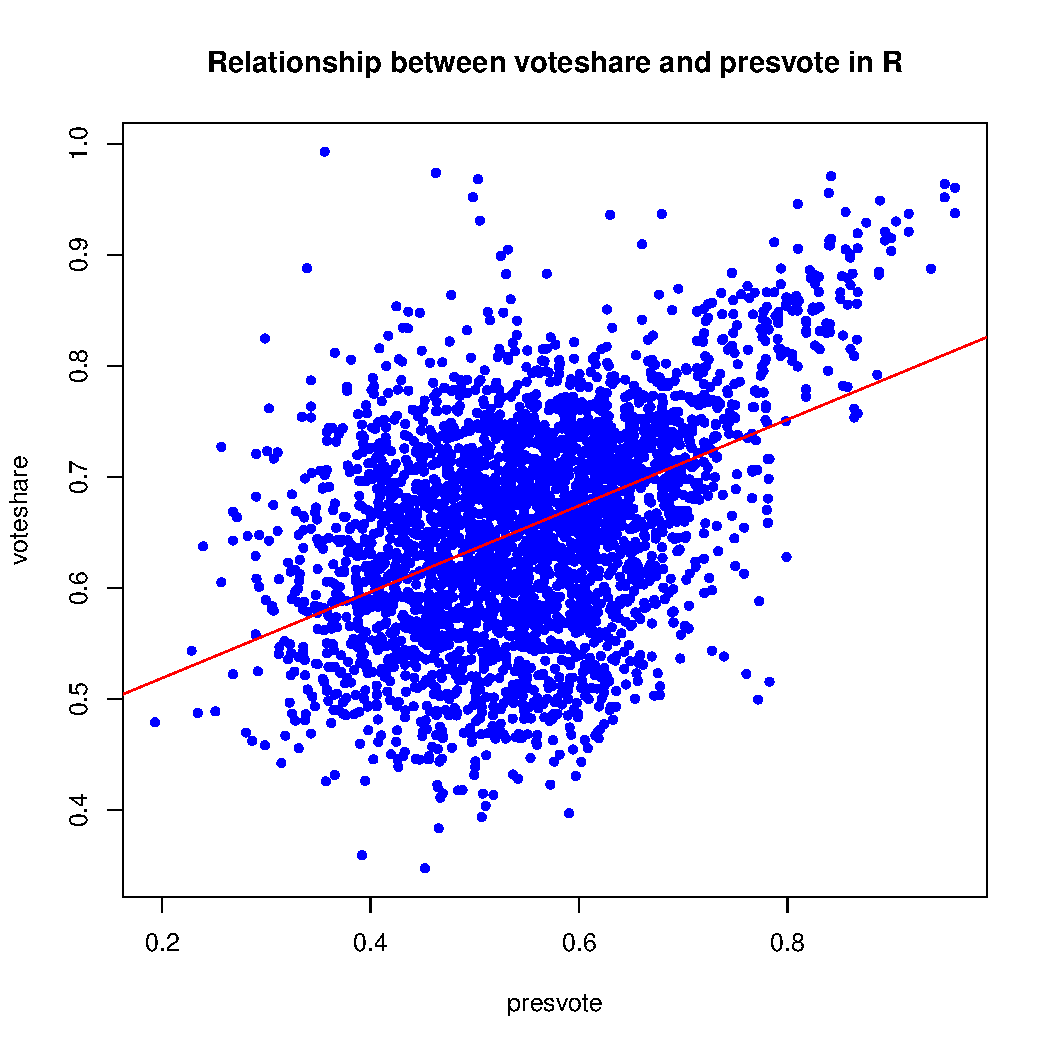
\includegraphics[width=0.8\textwidth]{Scatter plot and regression line of voteshare and presvote in R.pdf}
			\caption{Scatter plot and regression line of voteshare and presvote in R}
			\label{fig:pdf}
		\end{figure}
			\vspace{.15cm}
		
		\newpage	
		\item Write the prediction equation.\\
		\noindent \\From the results of regression3 in Part 3.1, we can get the intercept and slope respectively. So the prediction equation would be:\\  \[ \hat{\texttt{voteshare}}= 0.441330 + 0.388018*\texttt{presvote} \] \\ In this model, presvote has a positive effect on voteshare, the estimate value of voteshare would be 0.441330 when presvote is zero, with each addional unit change of presvote, the estimate voteshare changes by 0.388018.\\

	\end{enumerate}
	
	\newpage
\section*{Question 4}
\noindent The residuals from part (a) tell us how much of the variation in \texttt{voteshare} is $not$ explained by the difference in spending between incumbent and challenger. The residuals in part (b) tell us how much of the variation in \texttt{presvote} is $not$ explained by the difference in spending between incumbent and challenger in the district.
	\begin{enumerate}
		\item Run a regression where the outcome variable is the residuals from Question 1 and the explanatory variable is the residuals from Question 2.	\vspace{.16cm}
		
		 \noindent  We can use the lm() function in R to see the regression between \texttt{voteshare} and \texttt{presvote}. Run the following codes in R then we can get the results of regression4.	\vspace{.15cm}
		
		\lstinputlisting[language=R,firstline=111,lastline=113,]{PS3.R}
		
		\noindent We can get the following results: \vspace{.15cm}
		\begin{verbatim}
			Call:
			lm(formula = residuals_reg1 ~ residuals_reg2)
			Residuals:
			     Min       1Q   Median       3Q      Max 
			-0.25928 -0.04737 -0.00121  0.04618  0.33126 
			
			Coefficients: 
			                Estimate Std. Error t value Pr(>|t|)    
			(Intercept)    -1.942e-18  1.299e-03    0.00        1    
			residuals_reg2  2.569e-01  1.176e-02   21.84   <2e-16 ***
			---
			Signif. codes:  0 ‘***’ 0.001 ‘**’ 0.01 ‘*’ 0.05 ‘.’ 0.1 ‘ ’ 1
			
			Residual standard error: 0.07338 on 3191 degrees of freedom
			Multiple R-squared:   0.13,	Adjusted R-squared:  0.1298 
			F-statistic:   477 on 1 and 3191 DF,  p-value: < 2.2e-16
		\end{verbatim}
		\vspace{.15cm}
		
		\noindent From the results regression4 we can see that the P-value (\textless 2.2e-16) is extremely low, providing strong evidence in favor of a significant relationship between \texttt{residuals\textunderscore{}reg1} and \texttt{residuals\textunderscore{}reg2}\\ \vspace{.15cm}
		
		\item Make a scatterplot of the two residuals and add the regression line. 	\vspace{.16cm}
		
			\noindent First, we draw the scatter plot of the two variables, and then using the abline() function to add the regression line. By running the following codes in R. We can get the graphic.
		
		\lstinputlisting[language=R,firstline=116,lastline=125]{PS3.R}
		
		\begin{figure}[h]
			\centering
			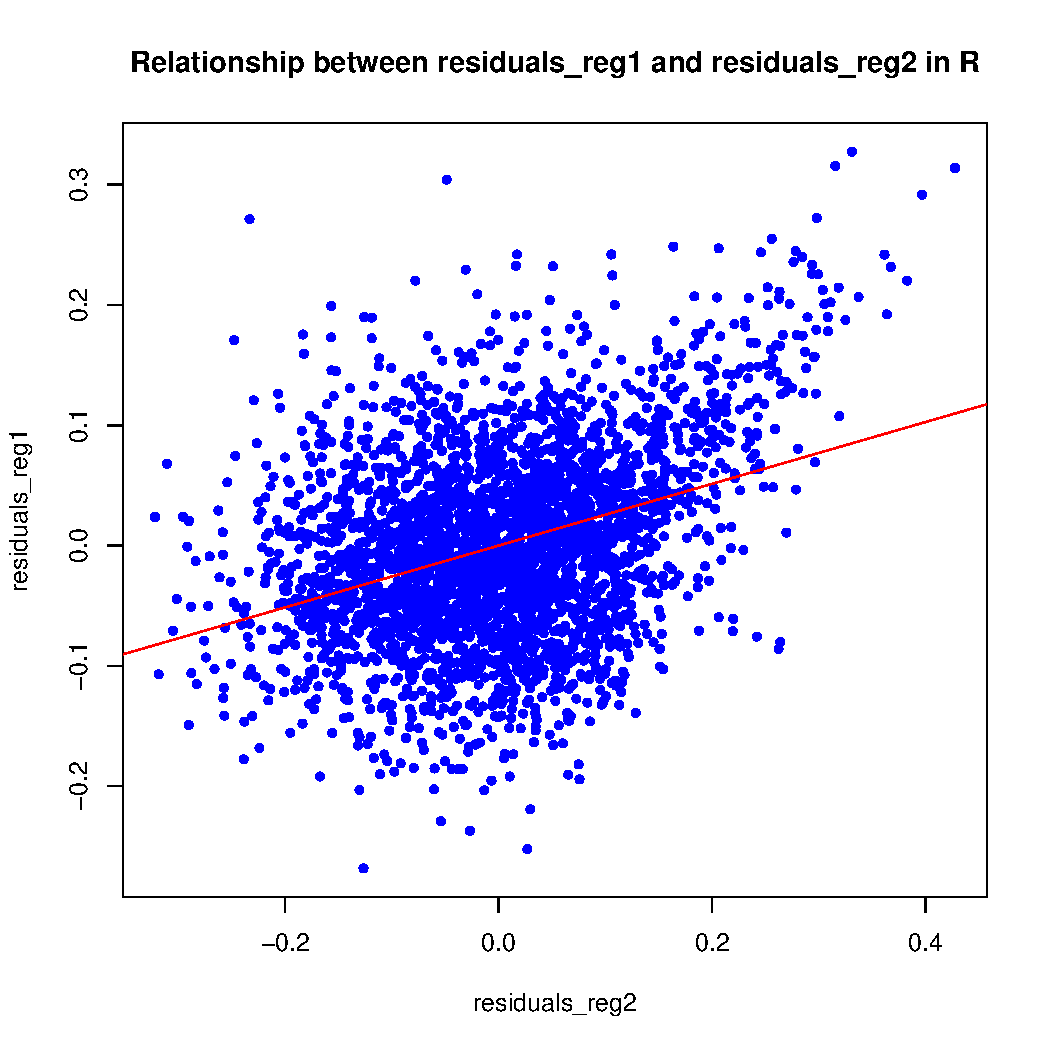
\includegraphics[width=0.8\textwidth]{Scatter plot and regression line of residuals_reg1 and residuals_reg2 in R.pdf}
			\caption{Scatter plot and regression line of residuals\textunderscore{}reg1 and residuals\textunderscore{}reg2 in R}
			\label{fig:pdf}
		\end{figure}
		\vspace{.15cm}
		
		\newpage
		\item Write the prediction equation.
		
		\noindent \\From the results of regression4 in Part 4.1, we can get the intercept and slope respectively. So the prediction equation would be:\\  \[ \hat{\texttt{residuals\textunderscore{}reg1}} = -1.942e-18 + (2.569e-01)*\texttt{residuals\textunderscore{}reg2} \]  \\In this model, residuals\textunderscore{}reg2 has a positive effect on residuals\textunderscore{}reg1, the estimate value of residuals\textunderscore{}reg1 would be -1.942e-18 when residuals\textunderscore{}reg2 is zero, with each addional unit change of residuals\textunderscore{}reg2, the estimate residuals\textunderscore{}reg1 changes by 2.569e-01.\\
		
	\end{enumerate}
	
	\newpage	

\section*{Question 5}
\noindent What if the incumbent's vote share is affected by both the president's popularity and the difference in spending between incumbent and challenger? 
	\begin{enumerate}
		\item Run a regression where the outcome variable is the incumbent's \texttt{voteshare} and the explanatory variables are \texttt{difflog} and \texttt{presvote}.	\vspace{.15cm}
		
		\noindent  We can use the lm() function in R to see the regression between \texttt{voteshare} , \texttt{difflog} and \texttt{presvote}. Run the following codes in R then we can get the results of regression5.	\vspace{.15cm}
		
		\lstinputlisting[language=R,firstline=132,lastline=134,]{PS3.R}
		
		\noindent We can get the following results: \vspace{.15cm}
		\begin{verbatim}
			Call:
			lm(formula = voteshare ~ difflog + presvote, data = inc.sub)
			
			Residuals: 
			    Min       1Q   Median       3Q      Max 
			-0.25928 -0.04737 -0.00121  0.04618  0.33126 
			
			Coefficients:
			             Estimate Std. Error t value Pr(>|t|)    
			(Intercept) 0.4486442  0.0063297   70.88   <2e-16 ***
			difflog     0.0355431  0.0009455   37.59   <2e-16 ***
			presvote    0.2568770  0.0117637   21.84   <2e-16 ***
			---
			Signif. codes:  0 ‘***’ 0.001 ‘**’ 0.01 ‘*’ 0.05 ‘.’ 0.1 ‘ ’ 1
			
			Residual standard error: 0.07339 on 3190 degrees of freedom
			Multiple R-squared:  0.4496,	Adjusted R-squared:  0.4493 
			F-statistic:  1303 on 2 and 3190 DF,  p-value: < 2.2e-16
		\end{verbatim}
		\vspace{.15cm}
		
		\noindent From the results regression5 we can see that the P-value (\textless 2.2e-16) is extremely low, providing strong evidence in favor of a significant relationship between \texttt{voteshare} , \texttt{difflog} and \texttt{presvote}\\ \vspace{.15cm}
		
		\newpage
		\item Write the prediction equation.	\vspace{.15cm}
		
		\noindent \\From the results of regression5 in Part 5.1, we can get the intercept and slopes respectively. So the prediction equation would be:\\  \[ \hat{\texttt{voteshare}} = 0.4486442 + 0.0355431*\texttt{difflog} + 0.2568770*\texttt{presvote} \]  \\In this model, both difflog and presvote have positive effects on voteshare, the estimate value of voteshare would be 0.4486442 when difflog and presvote are zero. Controlling presvote unchanged, with each addional unit change of difflog, the estimate voteshare changes by 0.0355431. Controlling difflog unchanged, with one unit presvote  increase, increasing the voteshare estimate by 0.2568770.\\
		
		\item What is it in this output that is identical to the output in Question 4? Why do you think this is the case?\\
		
		\noindent From the regression results of regression5 and regression4, we can see that the Residuals of regression4 and regression5 are the same.\\
		\\The reason for this situation is that the model of regression4 is obtained by regressing residuals\textunderscore{}reg1 on residuals\textunderscore{}reg2, while the model of regression5 is obtained by directly regressing voteshare on difflog and presvote. Since residuals\textunderscore{}reg1 and residuals\textunderscore{}reg2 are respectively the residuals of voteshare on difflog and the residuals of presvote on difflog, the residuals,  in the regression results will be the same. This is also why we see these same values in both regression results.
		
	\end{enumerate}




\end{document}
